
\chapter{Giải pháp đề xuất}
\label{chap:giai_phap_de_xuat}

Hệ thống chấm điểm phiếu trả lời trắc nghiệm tự động là một giải pháp công nghệ nhằm tối ưu hóa và chuẩn hóa quy trình đánh giá. Một hệ thống hoàn chỉnh thường bao gồm nhiều công đoạn, từ xử lý ảnh đầu vào đến việc xuất ra kết quả cuối cùng. Hình \ref{fig:tong_quan_he_thong_cham_diem} cung cấp một cái nhìn tổng quan về kiến trúc của một hệ thống.

\begin{figure}[H]
    \centering
    % \includegraphics[width=0.9\textwidth]{path/to/your/overall_grading_system_diagram.png}
        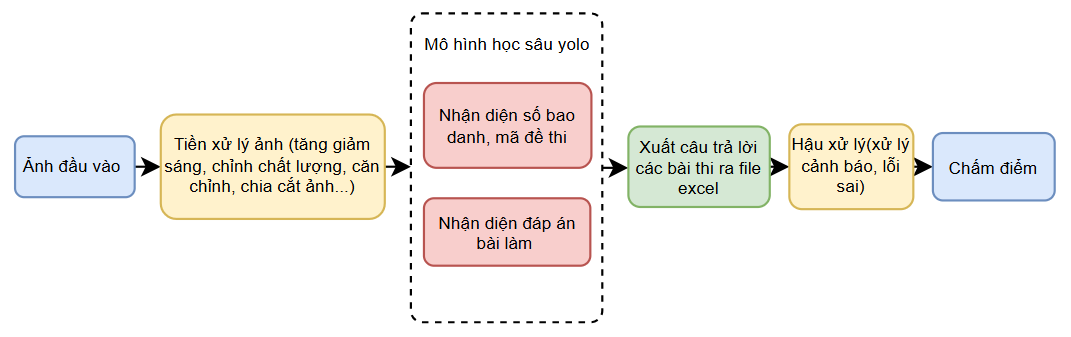
\includegraphics[width=1\textwidth]{img_proj/he_thong1.png}
    \caption{Sơ đồ kiến trúc tổng quan của một hệ thống chấm điểm trắc nghiệm tự động.}
    \label{fig:tong_quan_he_thong_cham_diem}
\end{figure}

Trong khuôn khổ của hệ thống tổng thể này,đồ án tập trung vào việc phát triển và đánh giá một thành phần then chốt: \textbf{mô-đun nhận diện đáp án bài làm} sử dụng mô hình học sâu yolov8. Thành phần này có nhiệm vụ tự động định vị và diễn giải các vùng nội dung quan trọng trên phiếu, bao gồm các ô lựa chọn đáp án, mã định danh thí sinh và mã đề thi. Mục tiêu là chuyển đổi dữ liệu hình ảnh thô thành thông tin có cấu trúc, làm đầu vào cho các khối xử lý tiếp theo như so khớp đáp án và tính điểm.

\section{Kiến trúc chi tiết của mô-đun nhận diện và trích xuất thông tin}
\label{sec:kien_truc_khoi_nhan_dien_trich_xuat}

Kiến trúc đề xuất cho mô-đun nhận diện và trích xuất thông tin được mô tả chi tiết hơn trong hình \ref{fig:kien_truc_chi_tiet_khoi_nhan_dien} và bao gồm các giai đoạn xử lý chính sau:

\begin{figure}[H]
    \centering
    % \includegraphics[width=0.8\textwidth]{path/to/your/detailed_module_architecture_diagram.png}
    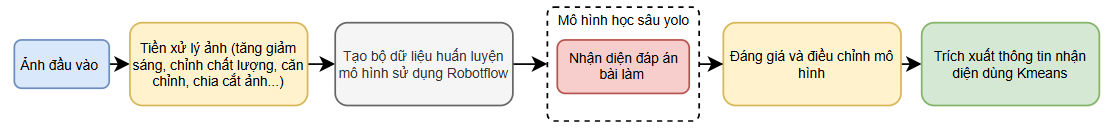
\includegraphics[width=1\textwidth]{img_proj/module_nhan_dang.png}
    \caption{Sơ đồ kiến trúc chi tiết của mô-đun Nhận Diện và Trích Xuất Thông Tin.}
    \label{fig:kien_truc_chi_tiet_khoi_nhan_dien}
\end{figure}

\begin{enumerate}
    \item \textbf{Tiền xử lý ảnh:}
    Ảnh phiếu đầu vào được xử lý để tối ưu hóa cho việc nhận diện. Các kỹ thuật như chuẩn hóa kích thước, tăng cường độ tương phản, hoặc loại bỏ nhiễu cục bộ có thể được áp dụng nhằm nâng cao chất lượng dữ liệu đầu vào cho mô hình.
    \item \textbf{Tạo tập dữ liệu huấn luận mô hình } sử dụng công cụ robotflow để gán nhãn cho những ảnh đã được xử lý đồng thời tăng cường và phân chia dữ liệu phục vụ huấn luyện mô hình.

    \item \textbf{Nhận diện đáp án bài làm bằng mô hình Học sâu:}
    Thành phần cốt lõi là mô hình mạng nơ-ron tích chập YOLOv8. Mô hình này, sau khi được huấn luyện trên một tập dữ liệu chuyên biệt, có khả năng định vị chính xác các ô tròn lựa chọn và các vùng chứa thông tin bài làm thông qua các hộp giới hạn. Quá trình huấn luyện và các khía cạnh kỹ thuật của mô hình sẽ được trình bày chi tiết trong mục \ref{sec:yolo_training_content_final}.

    \item \textbf{Hậu xử lý kết quả nhận diện và ánh xạ ô lựa chọn:}
    Các hộp giới hạn thu được từ mô hình YOLOv8 được xử lý tiếp. Đối với các ô tròn lựa chọn, thuật toán phân cụm K-means được sử dụng để nhóm các ô theo hàng (câu hỏi) và cột (lựa chọn), từ đó xác định vị trí logic của từng ô trên phiếu.

    \item \textbf{Trích xuất trạng thái ô lựa chọn và thông tin văn bản:}
    Sau khi ánh xạ, nội dung bên trong mỗi ô tròn được phân tích để xác định trạng thái "đã tô" hoặc "chưa tô".
\end{enumerate}

Kết quả đầu ra của khối này là một tập hợp dữ liệu có cấu trúc, bao gồm danh sách các lựa chọn đã được thí sinh tô chọn cho từng câu hỏi. Dữ liệu này sau đó sẽ được chuyển đến các khối tiếp theo trong hệ thống chấm điểm tổng thể để thực hiện việc so khớp đáp án và tính điểm.
\section{Phân tích thách thức và yêu cầu đối với mô-đun nhận diện}
\label{sec:thach_thuc_yeu_cau_module}

Việc phát triển một mô-đun nhận diện và trích xuất thông tin hiệu quả từ phiếu trả lời trắc nghiệm phải đối mặt với nhiều thách thức cố hữu và đòi hỏi các yêu cầu kỹ thuật cụ thể.

\subsection{Các thách thức chính trong nhận diện và trích xuất thông tin}
\label{ssec:thach_thuc_nhan_dien}

Quá trình tự động hóa việc "đọc" phiếu trắc nghiệm gặp phải các khó khăn sau:

\begin{itemize}
    \item \textbf{Tính đa dạng của dữ liệu đầu vào:}
    Chất lượng ảnh phiếu có thể thay đổi đáng kể do điều kiện quét hoặc chụp (độ phân giải, độ sáng, độ tương phản, độ nghiêng). Phiếu cũng có thể bị nhàu, có vết bẩn hoặc các dấu hiệu không mong muốn.

    \item \textbf{Sự biến thiên trong hành vi của người dùng:}
    Cách thí sinh tô các ô lựa chọn rất đa dạng: tô đậm, tô nhạt, tô không đầy ô, tô lem ra ngoài, sử dụng các loại bút khác nhau. Các trường hợp tẩy xóa và tô lại cũng tạo ra các mẫu hình phức tạp.

    \item \textbf{Độ phức tạp của cấu trúc phiếu:}
    Các ô lựa chọn thường nhỏ, nằm sát nhau và được bố trí theo một lưới dày đặc. Việc phân biệt chính xác từng ô riêng lẻ, cũng như định vị các vùng thông tin khác như số báo danh và mã đề, đòi hỏi độ phân giải và độ chính xác cao từ mô hình nhận diện.

    \item \textbf{Nhận diện và phân tách các đối tượng chồng chéo hoặc gần nhau:}
    Trong một số trường hợp, các ký tự hoặc đường kẻ trên phiếu có thể chạm vào hoặc chồng lấn một phần với các ô lựa chọn, gây khó khăn cho việc phân tách đối tượng.

    \item \textbf{Yêu cầu về tốc độ xử lý cho ứng dụng thực tế:}
    Mặc dù không phải là trọng tâm chính của giai đoạn phát triển mô hình, khả năng xử lý hiệu quả một lượng lớn phiếu vẫn là một yếu tố cần được cân nhắc cho các ứng dụng quy mô lớn.
\end{itemize}

\subsection{Yêu cầu đối với mô-đun nhận diện và trích xuất}
\label{ssec:yeu_cau_module}

Dựa trên các thách thức đã phân tích, mô-đun nhận diện và trích xuất thông tin cần đáp ứng các yêu cầu cốt lõi sau:

\begin{itemize}
    \item \textbf{Yêu cầu về chức năng nhận diện và trích xuất:}
    \begin{itemize}
        \item \textbf{Định vị chính xác các vùng quan tâm:} Mô-đun phải có khả năng tự động và chính xác định vị được vị trí (thông qua hộp giới hạn) của tất cả các ô tròn lựa chọn trên phiếu, cũng như các vùng chứa số báo danh và mã đề thi.
        \item \textbf{Ánh xạ logic các ô lựa chọn:} Phải có cơ chế để xác định mỗi ô tròn nhận diện được tương ứng với câu hỏi nào và lựa chọn (A, B, C, D,...) nào.
        \item \textbf{Trích xuất trạng thái ô lựa chọn:} Xác định một cách đáng tin cậy liệu một ô lựa chọn có được thí sinh tô chọn hay không.
        \item \textbf{Trích xuất thông tin văn bản (nếu có):} Có khả năng trích xuất nội dung ký tự từ các vùng số báo danh và mã đề.
    \end{itemize}

    \item \textbf{Yêu cầu về hiệu năng của mô hình nhận diện:}
    \begin{itemize}
        \item \textbf{Độ chính xác cao (high accuracy):} Tỷ lệ phát hiện đúng các đối tượng (true positives) phải cao, trong khi tỷ lệ phát hiện sai (false positives) và bỏ sót đối tượng (false negatives) phải ở mức tối thiểu. Các chỉ số như precision, recall, và mAP (mean average precision) là thước đo quan trọng.
        \item \textbf{Khả năng khái quát hóa tốt (good generalization):} Mô hình phải hoạt động hiệu quả trên các phiếu trắc nghiệm mới, chưa từng xuất hiện trong tập huấn luyện, bao gồm cả các biến thể về bố cục, chất lượng ảnh và cách tô đáp án.
        \item \textbf{Tính mạnh mẽ (robustness):} Mô hình cần có khả năng chịu đựng được một mức độ nhất định các yếu tố gây nhiễu và biến dạng trong dữ liệu đầu vào.
    \end{itemize}

    \item \textbf{Yêu cầu về dữ liệu cho phát triển mô hình:}
    \begin{itemize}
        \item \textbf{Dữ liệu huấn luyện đa dạng và đại diện:} Cần một bộ dữ liệu ảnh phiếu đã được gán nhãn chi tiết, bao phủ nhiều trường hợp và biến thể khác nhau để mô hình học được các đặc trưng một cách hiệu quả.
        \item \textbf{Quy trình gán nhãn nhất quán:} Đảm bảo chất lượng và tính nhất quán của các nhãn trong bộ dữ liệu huấn luyện.
    \end{itemize}
\end{itemize}

\section{Xây dựng và chuẩn hóa bộ dữ liệu huấn luyện}
\label{sec:xay_dung_chuan_hoa_du_lieu_v2}

Chất lượng và tính đại diện của bộ dữ liệu huấn luyện là yếu tố then chốt quyết định hiệu năng của hệ thống chấm trắc nghiệm tự động. Do đó, một quy trình xây dựng và chuẩn hóa dữ liệu được thiết kế một cách hệ thống và tỉ mỉ. Quy trình này bao gồm các giai đoạn chính: khởi đầu từ việc lựa chọn mẫu phiếu chuẩn và tạo dữ liệu mô phỏng đa dạng, tiếp nối bằng các bước tiền xử lý ảnh phức tạp, và kết thúc bằng việc gán nhãn chi tiết và tăng cường dữ liệu nhằm tối ưu hóa cho quá trình huấn luyện mô hình.

\subsection{Thiết lập dữ liệu gốc}
\label{subsec:du_lieu_goc_va_mo_phong_v2}

Nền tảng của bộ dữ liệu được xây dựng dựa trên một mẫu phiếu trả lời trắc nghiệm đã được định nghĩa trước, quy định rõ cấu trúc và vị trí các vùng thông tin thiết yếu. Để đảm bảo tính thực tiễn và nâng cao khả năng tổng quát hóa của mô hình, một khía cạnh quan trọng là việc mô phỏng các phương thức tô đáp án đa dạng mà sinh viên có thể thực hiện. Cụ thể, các phiếu mẫu được xử lý để bao gồm các kịch bản sau:
\begin{itemize}
    \item Các biến thể về độ đậm nhạt của nét tô: từ tô đậm rõ ràng đến tô mờ hoặc không đều mực.
    \item Các trường hợp tô không hoàn chỉnh: bao gồm tô một phần ô, tô lệch tâm.
    \item Tình huống tô lem mực ra ngoài phạm vi ô lựa chọn.
    \item Các phiếu có dấu hiệu tẩy xóa và chọn lại đáp án.
    \item Mô phỏng các khuyết điểm vật lý nhỏ trên phiếu: như bị nhàu nhẹ hoặc có vết bẩn không đáng kể.
\end{itemize}
Sau khi hoàn tất công đoạn mô phỏng này, toàn bộ các phiếu trả lời được quét (scan) thành các tệp ảnh số, lưu trữ với độ phân giải cao để bảo toàn chi tiết cho các giai đoạn xử lý kế tiếp.

\begin{figure}[H]
    \centering
    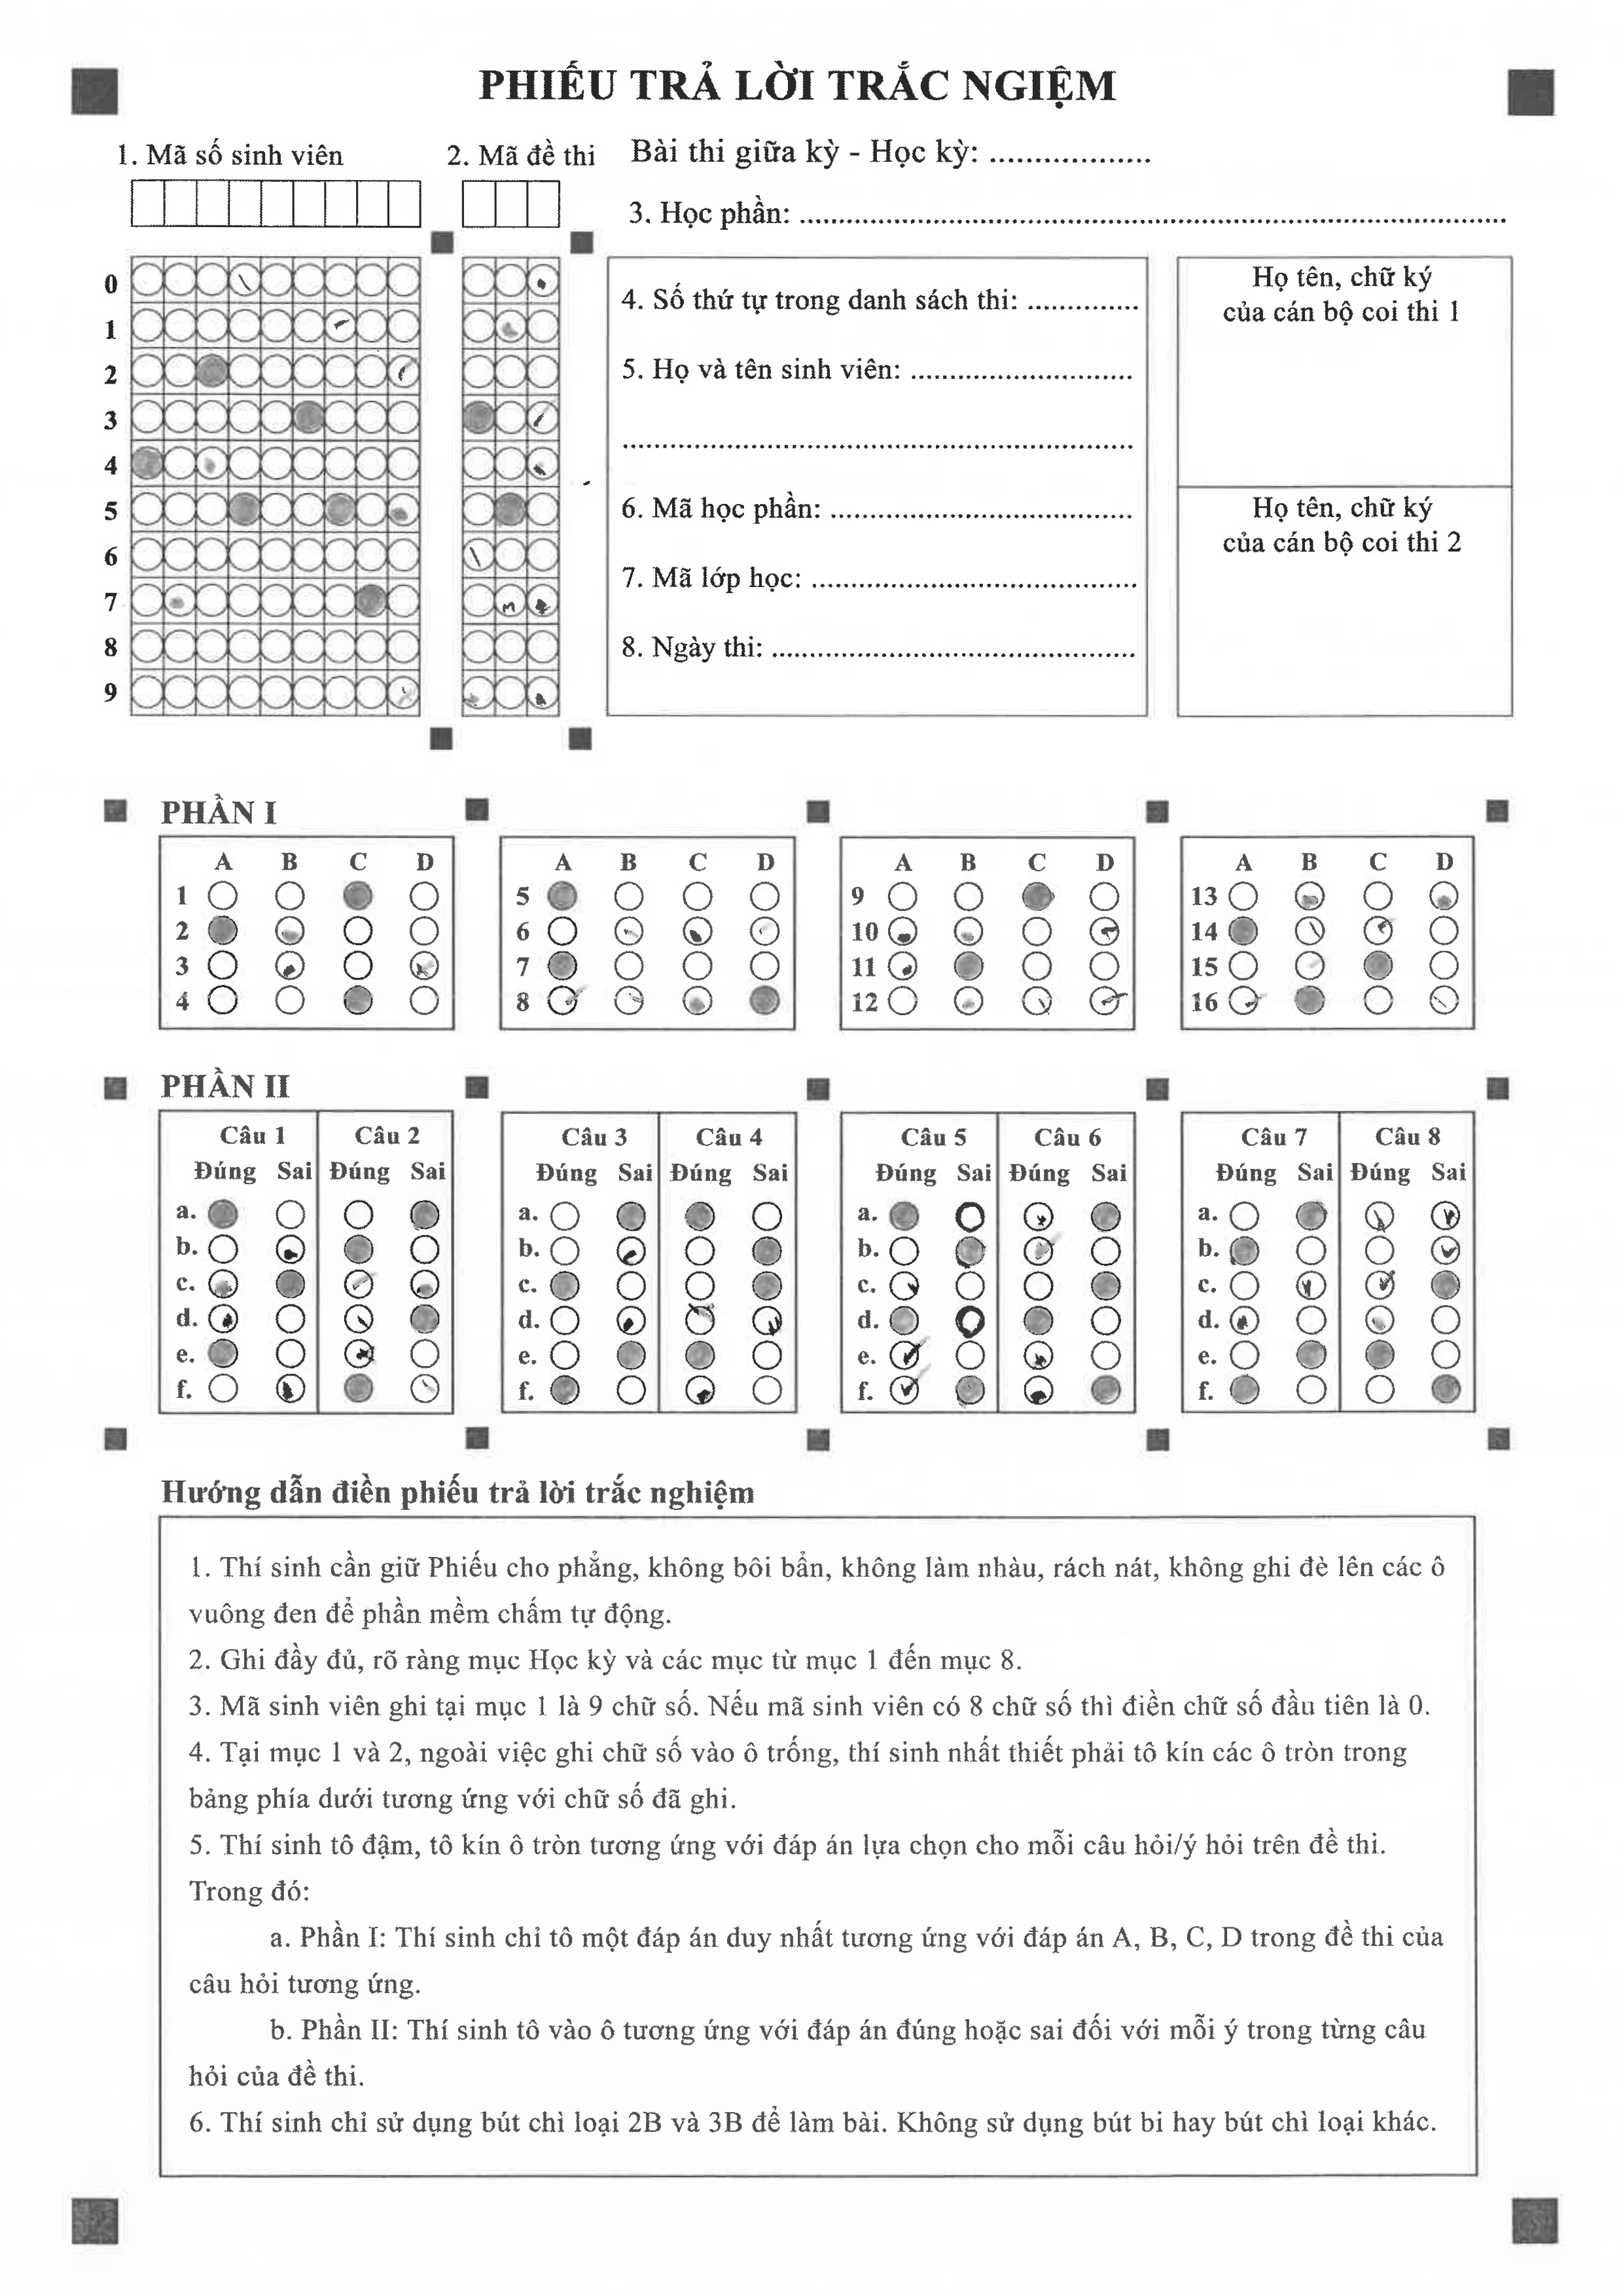
\includegraphics[width=0.8\textwidth]{img_proj/page_14.png}
    \caption{Minh họa phiếu trả lời được tô với các kịch bản đa dạng.}
    \label{fig:simulated_marking_revised_v2}
\end{figure}

\subsection{Tiền xử lý và chuẩn hóa ảnh quét}
\label{subsec:tien_xu_ly_anh_quet_with_templates_concise}

Ảnh quét thô thường chứa các biến dạng hình học và có sự khác biệt về đặc tính quang học, đòi hỏi các bước tiền xử lý để chuẩn bị dữ liệu đầu vào tối ưu cho mô hình nhận diện. Quy trình này bao gồm các giai đoạn chính:

\begin{enumerate}
    \item \textbf{Cải thiện chất lượng ảnh:}
    Để tăng cường độ tương phản và làm nổi bật các chi tiết quan trọng trên phiếu, các kỹ thuật điều chỉnh phân bố cường độ sáng, bao gồm hiệu chỉnh gamma \citep{Poynton1996}, được áp dụng. Bước này giúp nâng cao chất lượng hình ảnh cho các giai đoạn xử lý tiếp theo.

    \item \textbf{Căn chỉnh hình học ảnh:}
    Nhằm đảm bảo tính nhất quán về vị trí và góc xoay giữa các ảnh quét, ảnh đầu vào được căn chỉnh hình học so với một mẫu phiếu tham chiếu. Quy trình này dựa vào việc phát hiện các điểm đặc trưng bất biến theo tỷ lệ (thông qua SIFT \citep{Lowe2004}), sau đó tìm các cặp điểm tương ứng (với FLANN \citep{Muja2009}) và ước lượng phép biến đổi hình học (như ma trận homography thông qua RANSAC \citep{Fischler1981}) để hiệu chỉnh ảnh.

    \item \textbf{Định vị và trích xuất các vùng quan tâm:}
    Sau khi căn chỉnh, các khu vực chứa thông tin bài làm (các khối câu trả lời Phần I, Phần II) được tự động xác định và trích xuất. Kỹ thuật khớp mẫu (template matching) \citep{Brunelli2009TemplateMatching}, sử dụng các mẫu tham chiếu định trước (Hình \ref{fig:templates_for_matching_concise}) và các thước đo tương đồng như hệ số tương quan chuẩn hóa chéo, là một phương pháp được ứng dụng để định vị chính xác các vùng này. Kết quả của quá trình định vị được minh họa trong Hình \ref{fig:template_matching_result_concise}.

    \item \textbf{Chuẩn hóa Kích thước Ảnh Con:}
    Các ảnh con chứa vùng bài làm, sau khi được trích xuất, sẽ được chuẩn hóa về một kích thước đồng nhất (640x640 pixels). Quá trình này bao gồm việc thay đổi kích thước và có thể kèm theo việc đệm (padding) để đảm bảo tất cả ảnh đầu vào cho mô hình nhận diện có cùng kích thước và tỷ lệ khung hình.
\end{enumerate}

\begin{figure}[htbp] % Hình chứa 2 template
    \centering
    \begin{minipage}{0.45\textwidth} % Điều chỉnh kích thước và khoảng cách nếu cần
        \centering
        \includegraphics[width=0.25\linewidth]{small_template.png} % Giả sử width phù hợp
        \caption{Mẫu tham chiếu nhỏ.}
        \label{fig:small_template_concise}
    \end{minipage}\hfill % \hfill để tạo khoảng cách giữa hai minipage
    \begin{minipage}{0.45\textwidth}
        \centering
        
\includegraphics[width=0.5\linewidth]{big_template.png} % Giả sử width phù hợp
        \caption{Mẫu tham chiếu lớn.}
        \label{fig:big_template_concise}
    \end{minipage}
    \caption{Các mẫu tham chiếu (templates) được sử dụng trong kỹ thuật khớp mẫu để định vị vùng.}
    \label{fig:templates_for_matching_concise} % Label chung cho cả figure chứa 2 template
\end{figure}

\begin{figure}[htbp] % Hình kết quả khớp mẫu
    \centering
    \includegraphics[width=0.85\linewidth]{nem_form_result.png} % Điều chỉnh width nếu cần
    \caption{Kết quả định vị các vùng thông tin sau khi áp dụng kỹ thuật khớp mẫu.}
    \label{fig:template_matching_result_concise}
\end{figure}

Toàn bộ chuỗi tiền xử lý này nhằm mục đích tạo ra các ảnh đầu vào đồng nhất, đã được cải thiện về chất lượng và chuẩn hóa về kích thước, sẵn sàng cho giai đoạn huấn luyện và đánh giá mô hình nhận diện. Hình \ref{fig:preprocessing_example} tóm tắt các bước chính trong quy trình.

\begin{figure}[H] % Hoặc [htbp] để LaTeX linh hoạt hơn
    \centering
    \begin{minipage}{0.48\textwidth} % Chiếm khoảng 48% chiều rộng của text, có thể điều chỉnh
        \centering
        % Thay 'path/to/your/part1_processed.png' bằng đường dẫn và tên file thực của bạn
        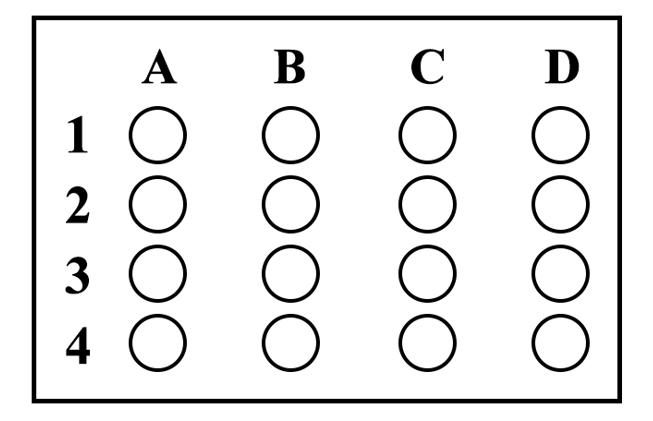
\includegraphics[width=\linewidth]{img_proj/a1.png}
        \caption*{(a) Vùng bài làm Phần I sau khi trích xuất và chuẩn hóa.} % \caption* để không có nhãn "Hình a:"
    \end{minipage}\hfill % Tạo khoảng cách ngang giữa hai minipage
    \begin{minipage}{0.48\textwidth}
        \centering
        % Thay 'path/to/your/part2_processed.png' bằng đường dẫn và tên file thực của bạn
        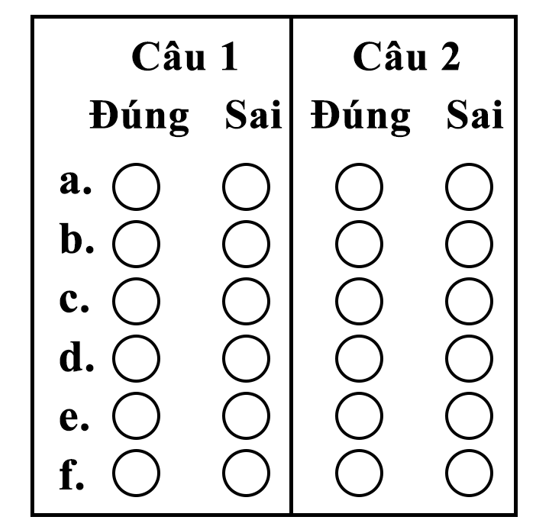
\includegraphics[width=\linewidth]{img_proj/a2.png}
        \caption*{(b) Vùng bài làm Phần II sau khi trích xuất và chuẩn hóa.}
    \end{minipage}
    \caption{Minh họa các vùng bài làm (Phần I và Phần II) sau khi được trích xuất và chuẩn hóa kích thước từ ảnh quét đã qua tiền xử lý.}
    \label{fig:extracted_and_normalized_parts} % Đặt label mới cho phù hợp
\end{figure}
\subsection{Xây dựng và gán nhãn bộ dữ liệu ảnh con với Roboflow}
\label{subsec:data_labeling_academic_condensed_2imgs_v6}

Sau giai đoạn tiền xử lý, việc xây dựng bộ dữ liệu có giám sát cho mô hình YOLO được tiến hành bằng nền tảng trực tuyến Roboflow. Nền tảng này cung cấp công cụ hiệu quả để định vị, phân loại và quản lý các đối tượng trong các ảnh con (vùng chứa các khối câu trả lời) đã được trích xuất và tải lên.

Chiến lược gán nhãn tập trung vào việc định vị từng ô lựa chọn đáp án và phân loại trực tiếp trạng thái của nó thành một trong hai lớp chính: \texttt{marked\_option} (lớp `1`, ô không tô) và \texttt{unmarked\_option} (lớp `0`, ô tô). Điều này cho phép mô hình YOLO học cách nhận diện đồng thời vị trí và đặc điểm trực quan của từng trạng thái ô.

Quy trình gán nhãn được triển khai theo phương pháp kết hợp, tối ưu hóa thời gian và chất lượng:
\begin{enumerate}
    \item \textbf{Gán nhãn thủ công ban đầu:} Một tập hợp con các ảnh được gán nhãn thủ công hoàn toàn trên Roboflow. Quá trình này bao gồm việc vẽ các hộp giới hạn (bounding boxes) chính xác quanh từng ô lựa chọn đáp án và gán lớp \texttt{marked\_option} hoặc \texttt{unmarked\_option} tương ứng, dựa trên đánh giá trực quan.
    % Hình ảnh 1 (trước là Hình 2): Minh họa cận cảnh việc gán nhãn thủ công một vài ô.
    \begin{figure}[H]
        \centering
        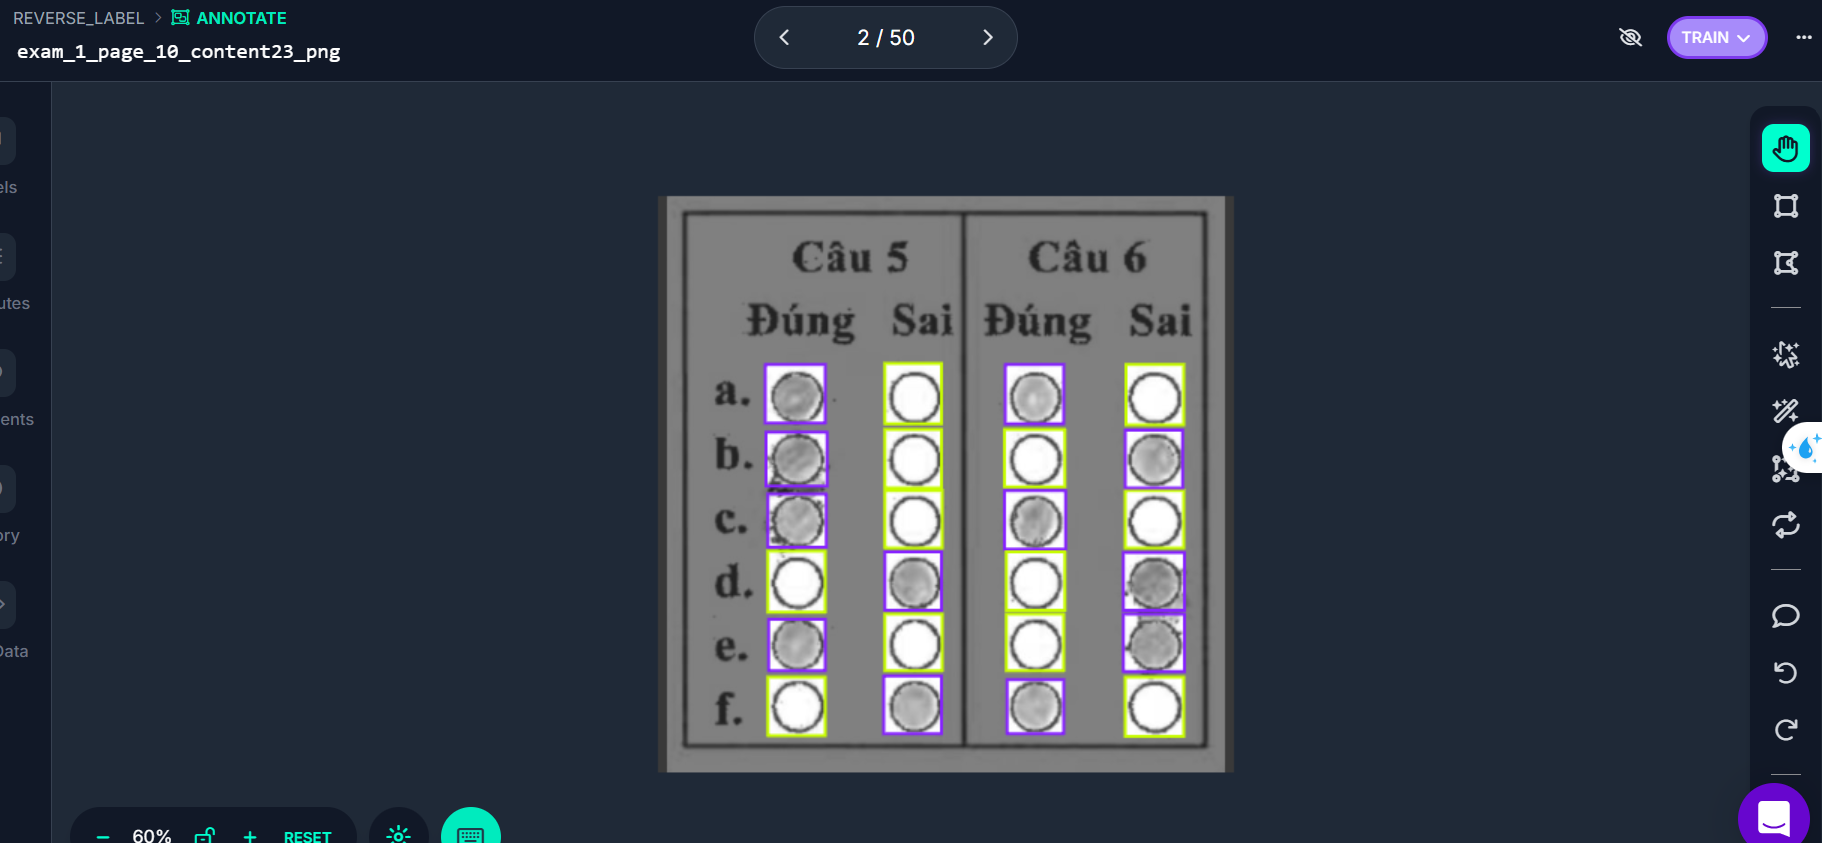
\includegraphics[width=0.8\textwidth]{img_proj/robo.png}
    
        \caption{Minh họa quy trình gán nhãn thủ công trên Roboflow}
        \label{fig:roboflow_manual_labeling_detail_v6}
    \end{figure}

    \item \textbf{Gán nhãn bán tự động với Mô hình Hỗ trợ:} Dữ liệu đã gán nhãn thủ công từ bước trên được sử dụng để huấn luyện một mô hình nhận diện đối tượng sơ bộ ngay trên nền tảng Roboflow. Mô hình này sau đó được triển khai như một công cụ hỗ trợ, tự động đề xuất các nhãn (hộp giới hạn và lớp) cho phần dữ liệu còn lại. Nhiệm vụ của người gán nhãn là rà soát, kiểm tra kỹ lưỡng và tinh chỉnh các nhãn do mô hình đề xuất để đảm bảo độ chính xác và nhất quán của toàn bộ bộ dữ liệu.
    % Hình ảnh 2 (trước là Hình 3): Giao diện Roboflow với các nhãn được model đề xuất.
    \begin{figure}[H]
        \centering
        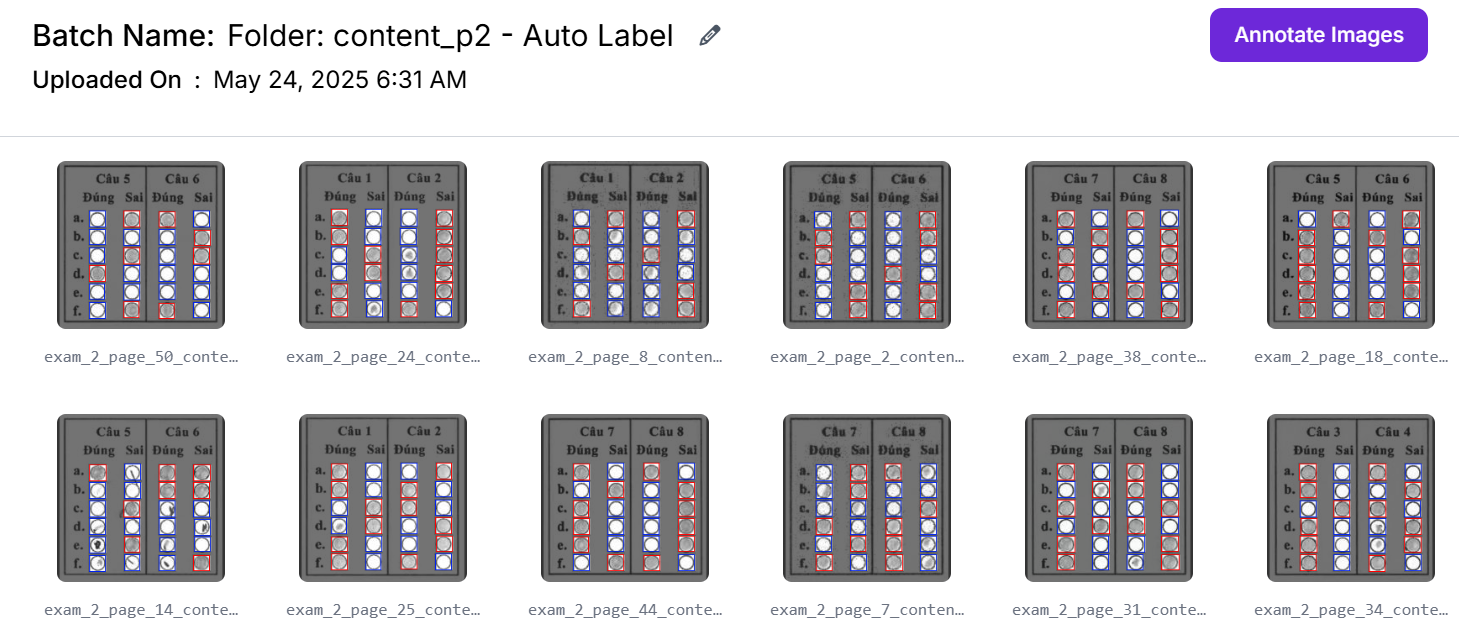
\includegraphics[width=0.8\textwidth]{img_proj/robo2.png}

        \caption{Mô hình hỗ trợ trên Roboflow để tăng tốc độ gán nhãn.}
        \label{fig:roboflow_model_assist_example_v6}
    \end{figure}
\end{enumerate}
Cách tiếp cận kết hợp này giúp giảm đáng kể thời gian và công sức so với việc thực hiện gán nhãn thủ công toàn bộ, đồng thời vẫn duy trì được chất lượng và độ tin cậy cao của dữ liệu huấn luyện nhờ vào bước kiểm tra và tinh chỉnh cuối cùng bởi con người.

Sau khi hoàn tất quá trình gán nhãn và các bước kiểm duyệt chất lượng, bộ dữ liệu được xuất từ Roboflow. Định dạng chuẩn của YOLO được lựa chọn, theo đó mỗi ảnh trong bộ dữ liệu sẽ có một tệp văn bản (\texttt{.txt}) tương ứng. Mỗi dòng trong tệp này đại diện cho một đối tượng đã được gán nhãn, chứa thông tin về ID của lớp (`0` cho \texttt{marked\_option}, `1` cho \texttt{unmarked\_option}) và bốn tọa độ chuẩn hóa của hộp giới hạn, sẵn sàng cho việc huấn luyện và đánh giá mô hình YOLO.
\subsection{Tăng cường dữ liệu}
\label{subsec:data_augmentation_specific_v3}

Nhằm mục đích gia tăng kích thước hiệu dụng và tính đa dạng của bộ dữ liệu huấn luyện, qua đó cải thiện khả năng tổng quát hóa của mô hình YOLO và giảm thiểu hiện tượng quá khớp (overfitting), các kỹ thuật tăng cường dữ liệu (Data Augmentation) đã được áp dụng một cách có hệ thống. Quá trình này được thực hiện thông qua các chức năng tích hợp sẵn trên nền tảng Roboflow, sau khi bộ dữ liệu gốc đã hoàn tất giai đoạn gán nhãn.

Chiến lược tăng cường dữ liệu được thiết kế để tạo ra các biến thể hợp lý từ mỗi ảnh huấn luyện gốc. Cụ thể, từ mỗi ảnh ban đầu, \textbf{ba phiên bản tăng cường} đã được tạo ra. Các phép biến đổi được lựa chọn và áp dụng một cách ngẫu nhiên hoặc theo một tỷ lệ xác định, tập trung chủ yếu vào các biến đổi quang học (photometric transformations) nhằm mô phỏng sự đa dạng về điều kiện thu nhận ảnh trong thực tế. Các kỹ thuật tăng cường chính được triển khai bao gồm:

\begin{itemize}
    \item \textbf{Chuyển đổi sang ảnh xám (Grayscale Conversion):} Một tỷ lệ 15\% trong số các ảnh được tạo ra đã được chuyển đổi sang định dạng ảnh xám. Kỹ thuật này giúp mô hình giảm sự phụ thuộc vào thông tin màu sắc và tập trung hơn vào các đặc trưng hình dạng và cấu trúc.
    \item \textbf{Điều chỉnh độ bão hòa màu (Saturation Adjustment):} Giá trị độ bão hòa màu của ảnh được thay đổi ngẫu nhiên trong một khoảng xác định, cụ thể là từ $-25\%$ đến $+25\%$ so với giá trị gốc. Phép biến đổi này mô phỏng sự thay đổi về độ rực rỡ của màu sắc do các yếu tố như chất lượng máy ảnh hoặc điều kiện ánh sáng.
    \item \textbf{Thay đổi độ sáng (Brightness Modification):} Độ sáng tổng thể của ảnh được điều chỉnh ngẫu nhiên trong phạm vi từ $-15\%$ đến $+15\%$. Điều này giúp mô hình trở nên kháng tốt hơn với các biến thể về cường độ ánh sáng chung của môi trường.
    \item \textbf{Điều chỉnh độ phơi sáng (Exposure Variation):} Giá trị phơi sáng của ảnh được biến đổi trong khoảng từ $-10\%$ đến $+10\%$. Kỹ thuật này mô phỏng các tình huống ảnh bị thiếu sáng hoặc thừa sáng nhẹ, tăng cường khả năng thích ứng của mô hình.
\end{itemize}

Các ảnh mới được tạo ra từ quá trình tăng cường này, cùng với các tệp nhãn YOLO tương ứng, kỳ vọng sẽ đóng góp vào việc xây dựng một mô hình YOLO mạnh mẽ và có khả năng hoạt động tốt trên các dữ liệu chưa từng thấy.

% Gợi ý hình ảnh: Một collage nhỏ gồm ảnh gốc và 3-4 ví dụ ảnh đã được tăng cường bằng các kỹ thuật bạn mô tả.
\begin{figure}[H] % Môi trường figure vẫn hữu ích để nhóm và căn giữa
    \centering
    % Ảnh 1: Điều chỉnh độ sáng
    \begin{minipage}[t]{0.32\textwidth}
        \centering
        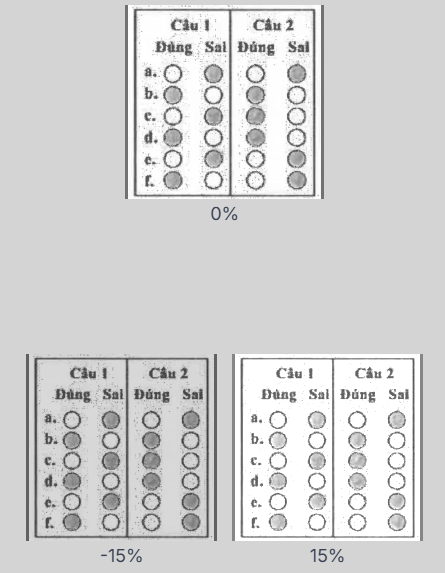
\includegraphics[width=\linewidth]{img_proj/ro1.png}
        \caption{Điều chỉnh độ sáng}
        % Bạn vẫn có thể thêm label ở đây nếu muốn tham chiếu đến nó, 
        % dù không có caption chính
        \label{fig:brightness_adj} 
    \end{minipage}
    \hfill
    % Ảnh 2: Điều chỉnh độ phơi sáng
    \begin{minipage}[t]{0.32\textwidth}
        \centering
        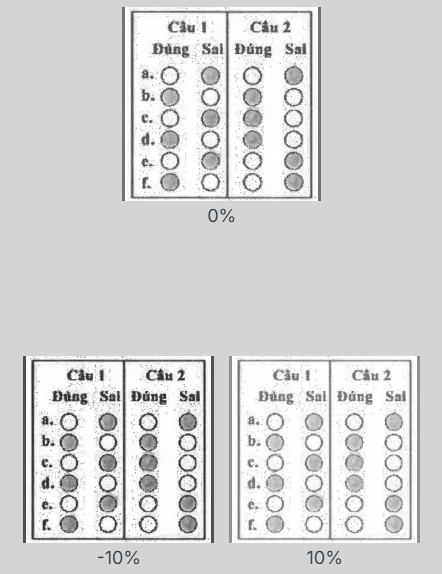
\includegraphics[width=\linewidth]{img_proj/ro2.png}
        \caption{Điều chỉnh độ phơi sáng}
        \label{fig:exposure_adj}
    \end{minipage}
    \hfill
    % Ảnh 3: Điều chỉnh độ bão hòa màu
    \begin{minipage}[t]{0.32\textwidth}
        \centering
        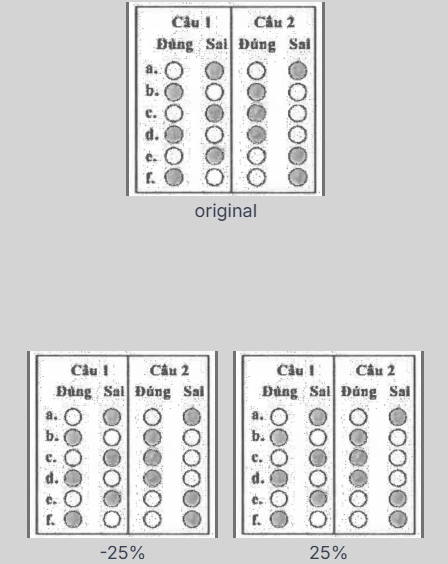
\includegraphics[width=\linewidth]{img_proj/ro3.png}
        \caption{Điều chỉnh độ bão hòa màu}
        \label{fig:saturation_adj}
    \end{minipage}

    % Không có \caption và \label cho cả figure ở đây nữa
    % \caption{Tăng cường dữ liệu: c) điều chỉnh độ sáng, d) điều chỉnh độ phơi sáng, và e) điều chỉnh độ bão hòa màu.}
    % \label{fig:specific_data_augmentation_examples_v3}
\end{figure}
\subsection{Phân chia tập dữ liệu cho huấn luyện và đánh giá Mô hình}
\label{subsec:phan_chia_du_lieu_final} % Label ngắn gọn hơn một chút

Sau các bước chuẩn bị và tăng cường, bộ dữ liệu cuối cùng bao gồm 1561 ảnh. Trước khi tiến hành phân chia, một bước tiền xử lý bổ sung được thực hiện thông qua các tùy chọn của công cụ Roboflow:
\begin{itemize} % nosep (từ enumitem) để giảm khoảng cách giữa các item
    \item \textbf{Tự động điều chỉnh độ tương phản (Auto-Adjust Contrast):} Phương pháp \textbf{Contrast Stretching} được áp dụng để tăng cường độ tương phản của hình ảnh, qua đó cải thiện chất lượng dữ liệu đầu vào cho mô hình.
\end{itemize}

Để đảm bảo quá trình huấn luyện và đánh giá mô hình diễn ra một cách khách quan, đồng thời giúp phát hiện và hạn chế hiện tượng quá khớp (overfitting), bộ dữ liệu này được phân chia thành ba tập con riêng biệt:
\begin{itemize}
    \item \textbf{Tập huấn luyện (Train set):} Chiếm tỷ lệ lớn nhất trong tổng số dữ liệu, được sử dụng trực tiếp để "dạy" mô hình và cập nhật các trọng số của nó (trong trường hợp này là mô hình YOLO).
    \item \textbf{Tập kiểm định (Validation set):} Một phần nhỏ hơn được dùng để theo dõi hiệu suất của mô hình trong suốt quá trình huấn luyện. Dữ liệu từ tập này đóng vai trò quan trọng trong việc tinh chỉnh các siêu tham số (hyperparameters) và áp dụng các chiến lược tối ưu hóa như dừng sớm (early stopping).
    \item \textbf{Tập kiểm thử (Test set):} Phần dữ liệu còn lại, được giữ hoàn toàn độc lập và chỉ được sử dụng một lần duy nhất sau khi mô hình đã hoàn tất quá trình huấn luyện. Mục đích của tập này là cung cấp một đánh giá khách quan và công bằng về khả năng tổng quát hóa của mô hình trên dữ liệu mới mà nó chưa từng gặp phải.
\end{itemize}

\begin{figure}[!htbp] % Sử dụng [!htbp] để LaTeX có nhiều lựa chọn vị trí hơn [h!]
    \centering
    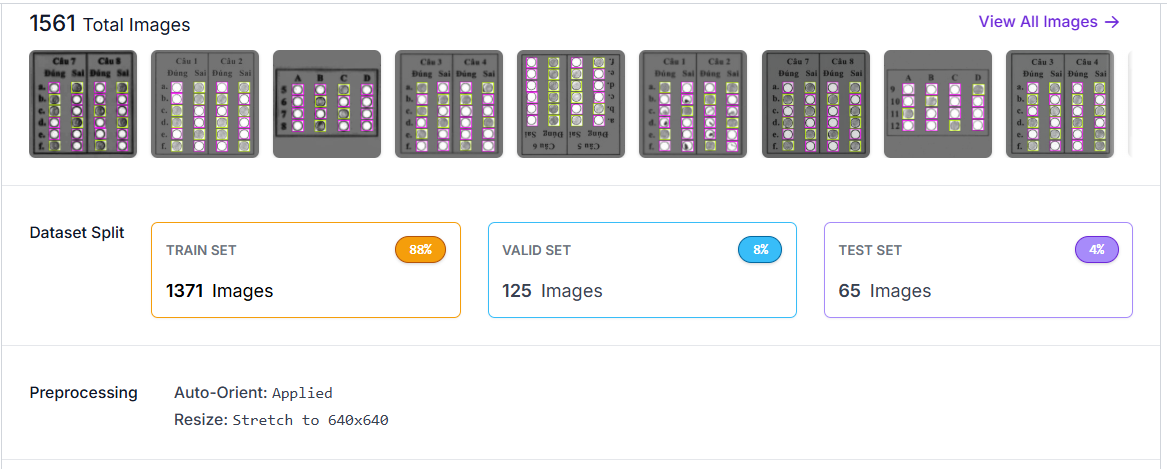
\includegraphics[width=0.8\linewidth]{img_proj/robo4.png}
    % Hãy thay "Caption mẫu..." bằng một chú thích cụ thể cho hình ảnh của bạn
    \caption{Phân chia tập dữ liệu.}
    \label{fig:dataset_split_visualization} % Một label mang tính mô tả hơn
\end{figure}

%--------------------------
\section{Xây dựng và huấn luyện mô hình nhận diện}
\label{sec:yolo_training_content_final}
Sau giai đoạn chuẩn bị dữ liệu, quy trình phát triển tập trung vào việc xây dựng và huấn luyện mô hình có khả năng nhận diện các thành phần cốt lõi trong nội dung bài làm. Dự án đã áp dụng kiến trúc YOLOv8, một lựa chọn được công nhận rộng rãi về hiệu năng và tính linh hoạt trong lĩnh vực thị giác máy tính.

\subsection{Lựa chọn kiến trúc mô hình: YOLOv8}
YOLO (You Only Look Once) là một dòng mô hình nhận diện đối tượng thời gian thực tiên tiến. Phiên bản YOLOv8, do Ultralytics phát triển, được chọn lựa nhờ những cải tiến đáng kể về độ chính xác và tốc độ so với các phiên bản tiền nhiệm. Đối với nhiệm vụ nhận diện các vùng nội dung trong bài thi, các ưu điểm của YOLOv8 trở nên đặc biệt hữu ích:
\begin{itemize}
    \item \textbf{Độ chính xác cao:} YOLOv8 thể hiện khả năng đạt được kết quả hàng đầu trên nhiều bộ dữ liệu benchmark.
    \item \textbf{Tốc độ xử lý ưu việt:} Đáp ứng yêu cầu xử lý nhanh của hệ thống chấm thi tự động.
    \item \textbf{Kiến trúc linh hoạt:} Cung cấp nhiều biến thể, cho phép cân nhắc giữa tốc độ và độ chính xác để chọn ra mô hình tối ưu cho tài nguyên và yêu cầu của dự án. Một biến thể phù hợp của YOLOv8 đã được triển khai, nhằm đạt được sự cân bằng hiệu quả giữa các yếu tố này.
    \item \textbf{Hệ sinh thái hỗ trợ mạnh mẽ:} Ultralytics cung cấp một framework toàn diện, tạo điều kiện thuận lợi cho việc huấn luyện, đánh giá và triển khai.
\end{itemize}

\subsection{Cấu hình mô hình nhận diện nội dung}
\label{subsec:model_config_content_final}
Việc thiết lập các tham số cấu hình đóng vai trò quyết định đến hiệu quả của mô hình. Các cấu hình chính cho mô hình nhận diện nội dung bài làm được xác định như sau:

\begin{itemize}
    \item \textbf{Mô hình nền tảng:} Một biến thể của kiến trúc YOLOv8 được sử dụng. Quá trình huấn luyện được khởi tạo từ các trọng số đã được tiền huấn luyện trên một bộ dữ liệu quy mô lớn. Phương pháp học chuyển giao (transfer learning) này giúp tăng tốc độ hội tụ và có khả năng cải thiện hiệu năng tổng thể.
    \item \textbf{Tệp cấu hình dữ liệu (\texttt{data.yaml}):} Tệp này quy định đường dẫn tới các tập dữ liệu huấn luyện, kiểm định, cùng số lượng và tên của các lớp đối tượng cần nhận diện. Đối với việc nhận diện các phần nội dung chính trong bài làm, cấu trúc tệp cấu hình được thiết lập như sau:
\begin{verbatim}
train: path/to/content_dataset/train/images
val: path/to/content_dataset/val/images
# test: path/to/content_dataset/test/images (Tùy chọn)

nc: 2 # Số lượng lớp đối tượng cho phần nội dung
names: ['content_part_1', 'content_part_2'] # Tên cụ thể của các lớp
\end{verbatim}
    Đường dẫn và tên lớp được điều chỉnh để phản ánh chính xác cấu trúc dữ liệu của dự án. Mô hình này tập trung vào 02 lớp đối tượng chính.
    \item \textbf{Các Siêu tham số huấn luyện chính (Key Hyperparameters):}
    \begin{itemize}
        \item \textbf{Kích thước lô (batch size):} \texttt{16}.
        \item \textbf{Số kỷ nguyên (epochs):} \texttt{200}. Quá trình huấn luyện được giám sát chặt chẽ, với cơ chế dừng sớm (early stopping patience: \texttt{20}) được áp dụng để tối ưu hóa thời gian và tài nguyên nếu không có cải thiện đáng kể trên tập kiểm định.
        \item \textbf{Kích thước ảnh đầu vào (image size - imgsz):} \texttt{640x640} pixels.
        \item \textbf{Tốc độ học ban đầu (initial learning rate - lr0):} \texttt{0.001}.
        \item \textbf{Thuật toán Tối ưu (optimizer):} Thuật toán tối ưu mặc định được đề xuất bởi framework YOLOv8, thường là AdamW, đã được sử dụng.
    \end{itemize}
\end{itemize}

\begin{figure}[h!]
    \centering
    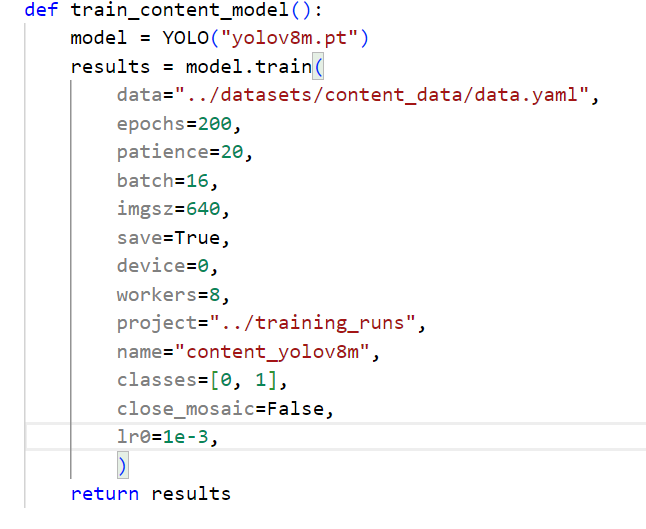
\includegraphics[width=0.7\linewidth]{img_proj/code_train.png}
    \caption{Siêu tham số huấn luyên mô hình}
    \label{fig:enter-label}
\end{figure}

\subsection{Quy trình huấn luyện mô hình}
\label{subsec:training_process_content_final}
Quá trình huấn luyện mô hình nhận diện nội dung được tiến hành bằng cách sử dụng API Python do Ultralytics cung cấp, cho phép kiểm soát chi tiết các tham số và tích hợp liền mạch vào luồng công việc của dự án.

\textbf{Triển khai huấn luyện:}
Mô hình được khởi tạo với các trọng số tiền huấn luyện và sau đó được tinh chỉnh (fine-tuned) trên bộ dữ liệu chuyên biệt cho việc nhận diện nội dung bài làm, tuân theo các siêu tham số đã được xác định tại mục \ref{subsec:model_config_content_final}.
\begin{itemize}
    \item \textbf{Dữ liệu đầu vào:} Bao gồm các tệp ảnh và tệp nhãn (annotations) tương ứng của các vùng nội dung bài làm. Dữ liệu này được tổ chức thành các tập huấn luyện và kiểm định theo khai báo trong tệp cấu hình dữ liệu.
    \item \textbf{Kết quả đầu ra:}
    \begin{itemize}
        \item Các tệp trọng số của mô hình, bao gồm trọng số tốt nhất (\texttt{best.pt}) và trọng số của epoch cuối cùng (\texttt{last.pt}). Các tệp này được lưu trữ trong một thư mục kết quả được chỉ định cho phiên huấn luyện.

    \end{itemize}
\end{itemize}


